\chapter{Die Realisierung}
\label{cha:Realisierung}
Folgendes Kapitel befasst sich mit der Implementierung, der im Kapitel \ref{cha:Lösungskonzept} vorgestellten Spezifikation des Vorlagenmanagements. Die Implementierung wurde in \emph{Java 8} mit dem \emph{Buildtool Maven} realisiert, wobei die Implementierungen in der folgenden Projektstruktur organisiert wurden.
\newline
\dirtree{%
.1 mailing.
.2 module.
.3 template.
.4 cdi.
.4 jsf.
.4 model.
.5 json.
.4 logic.
.5 api.
.5 impl.
.3 integration.
.4 clevercure-web.
.2 testsuite.
.3 cdi.
.2 demo.
.3 web.
.2 data.
.3 api.
.3 impl.
}
\ \newline
Das Wurzelprojekt \emph{mailing} organisiert alle Abhängigkeiten für die Unterprojekte sowie die gemeinsame \emph{Build}-Konfiguration, die auf alle konkreten Projekte angewendet werden kann. Ebenfalls enthält es die Metadaten wie die EntwicklerInnen, die an diesem Projekt mitwirken. Die Unterprojekte, die ebenfalls \emph{Paren}-Projekte bündeln ihre Unterprojekte und organisieren keine Abhängigkeiten und definieren keine Metadaten. Die gesamte Organisation findet im \emph{Paren}-Projekt \emph{mailing} statt. Diese Projektstruktur wurde gewählt, da in diesem Projekt in weitere Folge auch die Implementierungen der anderen benötigten Softwarekomponenten des \emph{Mail-Service} beinhalten wird. Die konkreten Artefakte wurden jeweils in ein Artefakt \emph{*-api} und \emph{*-impl} aufgeteilt, somit sind die Schnittstellen vollständig getrennt von der Implementierung.
\newline
\newline
Die folgenden Artefakte resultieren aus dieser Projektstruktur, wobei nur die konkreten Artefakte und nicht die \emph{Parent}-Artefakte angeführt sind.
\begin{itemize}
	\item\emph{\textbf{mailing-module-template-logic-api}} ist das Artefakt, das die Spezifikation des Vorlagenmanagement enthält.
	\item\emph{\textbf{mailing-module-template-logic-impl}} ist das Artefakt, das die Implementierung der Spezifikation des Vorlagenmanagements enthält.
	\item\emph{\textbf{mailing-module-template-cdi}} ist das Artefakt, das die Implementierung für die Integration in einen \emph{CDI-Container} enthält.
	\item\emph{\textbf{mailing-module-template-jsf}} ist das Artefakt, das die Implementierung für die Integartion in \emph{JSF} enthält.
	\item\emph{\textbf{mailing-module-template-model-json}} ist das Artefakt, das die Implementierung der \emph{JSON}-Spezifikation enthält.
	\item\emph{\textbf{mailing-module-integartion-clevercure-web}} ist das Artefakt, das die Implementierung der Integration für die Anwendung \emph{CleverWeb} enthält.
	\item\emph{\textbf{mailing-data-api}} ist das Artefakt, dass die Spezifikation der \emph{Services} enthält.
	\item\emph{\textbf{mailing-data-impl}} ist das Artefakt, das die Implementierung der \emph{Service}-Spezifikation enthält.
	\item\emph{\textbf{mailing-testsuite-cdi}} ist das Artefakt, das die Basis aller Tests, die in einem \emph{CDI-Container} lauffähig sein sollen darstellt.
	\item\emph{\textbf{mailing-demo-web}} ist das Artefakt, das die Demowebanwendung darstellt.
\end{itemize} 
\ \newline


\section{Die Implementierung der Spezifikationen}
Der folgende Abschnitt behandelt die Implementierungen der im Kapitel \ref{cha:Lösungskonzept} vorgestellten Spezifikation.

\subsection{Die Implementierung für \emph{CKEditor}}
\emph{CKEditor} ist ein \emph{Javascript} basierter mit dem die Vorlagen bearbeitet werden können. Wie in \ref{sec:sub-typescript-javascript} vorgegeben wird ein \emph{Plugin} benötigt, dass innerhalb des \emph{CKEDitor} die Variablen verwalten kann. Diese \emph{Plugin} wurde in \emph{Typescript} implementiert, da hier Typsicherheit vorhanden ist im Gegenzug zu Javascript das nicht typsicher ist. Die Implementierung des \emph{Plugins} in \emph{Typescript} war möglich, da für den \emph{CKEditor} Typinformationen für \emph{Typescript} vom dem \emph{Open-Source} Projekt \emph{DefinitelyTyped} bereitgestellt wird. \emph{Typescript} benötigt Typinformationen für \emph{Javascript} Quelltext, damit die Typsicherheit in \emph{Typescript} gewährleistet werden kann. Würden keine Typinformationen zur Verfügung stehen, hätte man sie selber implementieren müssen. 
\newline
\newline
Der Quelltext befindet sich zurzeit im Projekt \emph{mailing-demo-web}, da die Verwendung eines \emph{Web-Fragment} das Problem mit sich bringt, dass während der Entwicklung die Ressourcen nicht automatisch nachgeladen werden können, was die Entwicklung sehr erschwert. Da es sich aber nur um zwei Quelltexte handelt, die einfach verschoben werden können, stellt das kein Problem dar.
 
\subsubsection{Das \emph{CKEDitor-Plugin} in Typescript}
Da das Variablenmanagement unabhängig vom verwendeten \emph{CKEditor} ist, wurde die Verwaltung der Variablen in einem eigenen \emph{Javascript} Modul \emph{cc.variables} zusammengefasst. Das \emph{CKEditor Plugin} wurde im \emph{Javascript} Modul \emph{cc.ckeditor.plugins} zusammengefasst. Das Variablenmanagement in \emph{Typescript} ist verantwortlich für die \emph{Browser} seitige Registrierung der Variablen und stellt Hilfsmethoden zur Verfügung zur Verfügung, mit denen Variablen in der \emph{Registry} gefunden und konvertiert werden können. Folgendes Beispiel soll illustrieren wie eine Variable konvertiert werden kann.
\begin{JsCode}[numbers=none]
// Signature of the converter function
public convertVariables(converter:(item:VariableMapping) => any 
                        = (item:VariableMapping)=> item):any[]

// Convert to the variable's set displayName
variablesHandler.convertVariables(
	function (variable) {
		return variable.displayName;
	}
)                        
\end{JsCode}
Die Funktion \emph{convertVariables} definiert den Formalparameter \emph{converter} als eine sogenannte \emph{Arrow}-Funktion, die einer \emph{Lambda}-Funktion in \emph{Java} ähnelt. Mit der \emph{Arrow}-Funktion wird die Signatur der Funktion für die Konvertierung vorgegeben. Ebenfalls wird für den Formalparameter \emph{converter} eine Standardimplementierung definiert, die verwendet wird, sollte der Formalparameter \emph{converter} bei Aktivierung der Funktion \emph{convertVariables} nicht gesetzt sein. Der Typ \emph{any[]} ist vergleichbar mit dem Datentyp \emph{var} aus \emph{.NET} und gibt an das jeder Datentyp als Typ des zurückgelieferten \emph{Arrays} erlaubt ist.
\newline
\newline
Das \emph{CKEditor Plugin} ist für die Integration der Variablen in den \emph{Editor} verantwortlich, wobei die zur Verfügung stehenden Variablen über einen Dialog ausgewählt werden können. Ausgewählte Variablen werden an die aktuelle Position des Cursors im \emph{Editor} in Form eines \emph{HTML Tags} platziert. Die \emph{HTML}-Repräsentation der Variable ist gekoppelt an den \emph{FacesConverter}, da der Konverter die Variable von dessen \emph{HTML}-Repräsentation in die \emph{Template-Engine} spezifische Repräsentation überführen können muss. Die verwendete \emph{Template-Engine} ist für diese \emph{Plugin} irrelevant, da die Variablen immer in dieselbe \emph{JSON}-Repräsentation überführt werden.
\begin{figure}[h]
\centering
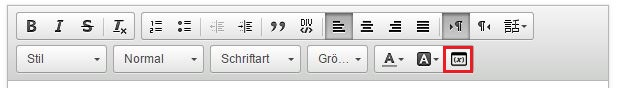
\includegraphics[scale=0.7]{ckeditor-toolbar-open-dialog}
\caption{\emph{CKEditor Toolbar Button} zum Öffnen des Dialogs}
\label{fig:ckeditor-toolbar-opne-dialog}
\end{figure}
\ \newline
Der in Abbildung \ref{fig:ckeditor-toolbar-opne-dialog} rot markierte \emph{Toolbar Button} wird über das \emph{Plugin} registriert und in die \emph{Toolbar} eingefügt. Über diesen \emph{Button} kann der Dialog für die Variablenauswahl geöffnet werden.
\begin{figure}[h]
\centering
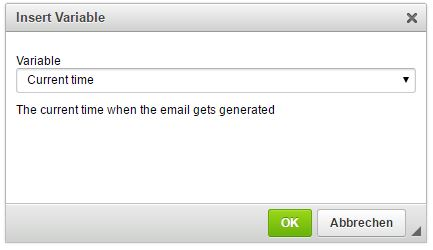
\includegraphics[scale=1]{ckeditor-dialog-insert-variable}
\caption{\emph{CKEditor} Dialog für die Variablenauswahl}
\label{fig:ckeditor-dialog-insert-variable}
\end{figure}
\ \newline
Über den Dialog aus Abbildung \ref{fig:ckeditor-dialog-insert-variable} stehen alle im \emph{CKEditor Plugin} registrierten Variablen zur Auswahl. Der Titel der Variable ist der Text in der Auswahlkomponente und die Beschreibung der ausgewählten Variable wird unterhalb der Auswahlkomponente angezeigt. Durch klick auf den \emph{Button OK} wird die Variable in die Vorlage eingefügt und der Dialog wird geschlossen.
\begin{figure}[h]
\centering
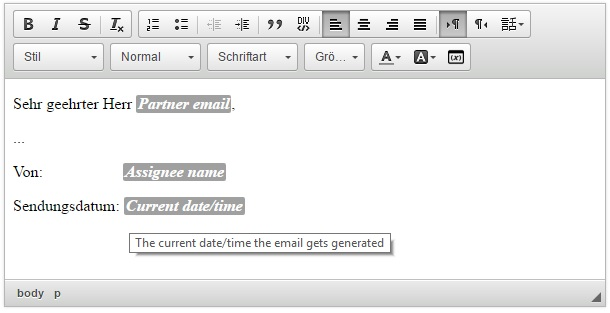
\includegraphics[scale=0.8]{ckeditor-example-template}
\caption{Beispiel einer Vorlage im \emph{CKEditor}}
\label{fig:ckeditor-example-template}
\end{figure}
\ \newline 
Die Abbildung \ref{fig:ckeditor-example-template} illustriert eine Vorlage innerhalb des \emph{CKEditors}, wobei die eingefügten Variablen besonders hervorgehoben werden. Der Titel der Variable stellt den Name für den \emph{HTML Tag} bereit und die Beschreibung dessen Titel. Die eingefügten \emph{HTML Tags} dürfen nicht verändert werden, daher ist das \emph{Drag and Drop} und das Selektieren dieses eingefügten Texts nicht erlaubt, da dadurch die \emph{HTML}-Repräsentation der Variablen zerstört werden könnte und die Variablen nicht mehr vom \emph{FacesConverter} gefunden werden können.
\newpage

\subsubsection{Die Variablenrepräsentation in JSON}
Die Variablen werden als Objekte der Schnittstelle \emph{VariableContract} definiert, und müssen für den \emph{CKEditor} in eine \emph{JSON}-Repräsentation überführt werden, die als \emph{Javascript}-Objekte innerhalb des \emph{CKEDitor Plugins} verwendet werden können. Dafür wurde in \emph{Typescript} eine Schnittstelle definiert, die die Struktur einer Variable innerhalb von \emph{Typescript} und \emph{Javascript} spezifiziert.
\begin{JsCode}[numbers=none]
module cc.variables {

    export interface VariableMapping {
    
        id:string,
        
        displayName:string,
        
        info:string,
    }
    
    ...
}
\end{JsCode}
\ \newline
Diese Schnittstelle ist Teil des Moduls \emph{cc.variables} und wird mit dem Schlüsselwort \emph{export} nach außen offengelegt und kann über den vollständigen Pfad \emph{cc.variables.VariableMapping} innerhalb von \emph{Typescript} und \emph{Javascript} verwendet werden. Mit dieser Schnittstelle werden Typinformationen für \emph{Typescript} bereitgestellt, die innerhalb von \emph{Typescript} die Typsicherheit sicherstellen. Solange die Variablen, die registriert werden, dieser Spezifikation folgen, können innerhalb des \emph{Typescipt} Quelltext keine Fehler auftreten.
\newline
\newline
Der Quelltext aus \ref{prog:variableJson} zeigt die Implementierung der \emph{JSON}-Spezifikation in \emph{Java}, die dazu verwendet wird, die Variablen in den spezifizierten \emph{JSON-String} zu überführen. Damit wird sichergestellt, das die Variablen in \emph{Typescript} korrekt registriert werden. Als \emph{JSON Provider} wird die Bibliothek \emph{fasterxml-jackson-json} vormals \emph{jackson-json} verwendet, die es erlaubt mit Annotationen deklarativ Attribute und/oder Methoden einer Klasse auf \emph{JSON}-Attribute abzubilden. Durch diesen deklarativen Ansatz sind die Attribute und/oder die Methoden einer Klasse entkoppelt von der \emph{JSON}-Spezifikation und können daher abgeändert werden. Nur ein Ändern des Datentyps eines Attributes könnte zu Problemen führen. 
\begin{program}
\caption{VariableJson.java}
\label{prog:variableJson}
\begin{JsCode}
@JsonTypeName(value = "variable-json")
public class VariableJson extends AbstractJsonModel {

    private String id;
    private String label;
    private String info;

    public VariableJson() {
    }

    public VariableJson(String id,
                        String displayName,
                        String tooltip) {
        this.id = id;
        this.label = displayName;
        this.info = tooltip;
    }

    @JsonGetter("id")
    public String getId() {
        return id;
    }

    @JsonSetter("id")
    public void setId(String id) {
        this.id = id;
    }

    @JsonGetter("displayName")
    public String getLabel() {
        return label;
    }

    @JsonSetter("displayName")
    public void setLabel(String label) {
        this.label = label;
    }

    @JsonGetter("info")
    public String getInfo() {
        return info;
    }

    @JsonSetter("info")
    public void setInfo(String info) {
        this.info = info;
    }
    
}
\end{JsCode}
\end{program}
\ \newpage


\subsection{Die Implementierungen für CDI}
Folgender Abschnitt behandelt die Implementierungen für die Integration in einen \emph{CDI Container}. Wie in Abschnitt \ref{sec:sub-template-management-cdi} beschrieben sollen die Variablen automatisch beim start des \emph{CDI Containers} registriert werden, sowie Vorlagenmanagementressourcen kontextabhängig über eine \emph{CDI Producer} zur Verfügung gestellt werden können. 

\subsubsection{Die Vorlagen-\emph{Management CDI-Extension}}
Um die Variablen beim Start des \emph{CDI Containers} automatisch registrieren zu können, wurde die Klasse \emph{TemplateCdiExtension} implementiert, die in der Lage ist auf Lebenszyklus \emph{Events} des \emph{CDI -Containers} zu reagieren und die Schnittstelle \emph{javax.enterprise.inject.spi.Extension} implementiert. Die Schnittstelle \emph{javax.enterprise.inject.spi.Extension} enthält keine abstrakten Methoden und markiert ein Implementierung als eine \emph{CDI-Extension}. Die \emph{CDI-Extension} wird als \emph{Service Provider} über die Schnittstelle \emph{Service-Provider-Interface} (SPI) registriert, in dem man eine folgende Datei erstellt \emph{META-INF/services/javax.enterprise.inject.spi.Extension}, die eine normale Textdatei ist und den vollständigen Namen der \emph{Service Provider} Implementierung enthält. 
\newline
\newline
Eine \emph{CDI-Extension} ist eigentlich kein \emph{CDI-Bean}, da ein Objekt der \emph{CDI-Extension} bereits beim Start des \emph{CDI-Containers} erstellt wird und somit existiert bevor der \emph{CDI-Container} vollständig gestartet ist. Trotzdem ist eine Extension injizierbar und kann in \emph{CDI-Beans} verwendet werden.
 
%\subsubsection{Der Vorlagen-\emph{Management CDI-Producer}}

%\subsubsection{Die Vorlagen-\emph{Management CDI-Utility}}


%\subsection{Die Implementierungen für JSF}

%\subsubsection{Der Vorlagen \emph{FacesConverter}}

%\subsubsection{Die \emph{Primefaces-Extension} für den \emph{CKEditor}}


%\section{Die Vorlagen-\emph{Management} Beispielanwendung}
%\subsection{Die Verwendung in einem \emph{Business}-Service}
%\subsection{Die Verwendung in der \emph{Web}-Oberfläche}